\documentclass[11pt,a4paper]{article}
\usepackage[margin=2.5cm]{geometry}
\usepackage{amsmath,amssymb}
\usepackage{booktabs}
\usepackage{graphicx}
\usepackage{caption}
\usepackage[numbers]{natbib}
\usepackage[hidelinks]{hyperref}
\graphicspath{{../figures/}}
\captionsetup{font=small,labelfont=bf}

\newcommand{\xbar}{\bar x}

\title{\textbf{Predatory Trading}\\[0.3em]
  \large Replicating, verifying and extending Brunnermeier \& Pedersen (2005)}
\author{Harsh Gupta \quad (22IM3FP29)\\[0.3em]
  \small Market Microstructure \quad$\cdot$\quad Prof.\ Ajay Kumar Mishra\\
  \small Indian Institute of Technology Kharagpur}
\date{October 2026}

\begin{document}
\maketitle

\begin{abstract}
\noindent
Brunnermeier and Pedersen (2005) show that when a large trader is forced to liquidate and
other large traders know it, those traders sell alongside it and buy back later, so the
price overshoots and liquidity disappears exactly when it is needed. We implement the model
as an exact discrete-time simulation and reproduce its propositions and figures. We then
check the equilibria independently: a linear-programming best-response solver finds no
profitable deviation from the paper's strategies, and traders starting from a naive
strategy learn the predatory equilibrium by fictitious play. Finally we use the same tools
for three extensions: collusion among predators, contagion with numerically computed
survival hurdles, and predators with unequal positions. The code, an interactive app and
115 automated tests are available at \url{https://github.com/dudegladiator/predatory-trading}.
\end{abstract}

% =========================================================================
\section{Introduction}

Large traders fear forced liquidation, especially when their need to sell is known to
others. Brunnermeier and Pedersen \cite{bp2005} (henceforth BP) model this situation and
call the response \emph{predatory trading}: trading that induces or exploits another
investor's need to reduce a position. Their motivating examples include the collapse of
Long-Term Capital Management in 1998, when counterparties allegedly sold the assets LTCM
had to sell, and the 1987 crash, when aggressive traders sold ahead of portfolio insurers.

The central result is counter-intuitive. One might expect rivals of a distressed trader to
provide liquidity by buying its shares cheaply. Instead they first \emph{sell} with it,
pushing the price below its new long-run level, and then buy back at the bottom. The
distressed trader's extra loss is exactly the predators' profit.

This report does three things.
\begin{enumerate}
  \item \textbf{Replication} (Section~\ref{sec:replication}). We build an exact
        discrete-time simulator of the model and reproduce BP's Propositions~1--9 and
        Figures~1--3 to the paper's printed precision.
  \item \textbf{Verification} (Section~\ref{sec:verification}). BP derive the
        equilibria analytically. We check them numerically and independently: best
        responses are linear programs, and none improves on BP's strategies. We also show
        that traders who start without any predation learn it on their own.
  \item \textbf{Extensions} (Section~\ref{sec:extensions}). Using the same tools we study
        three questions the paper raises but does not quantify: how much worse collusion
        makes predation and whether it is stable; how contagion spreads when survival
        hurdles are computed rather than assumed; and what drives overshooting when
        predators hold unequal positions.
\end{enumerate}

% =========================================================================
\section{The model}
\label{sec:model}

\subsection{Setting}
There is a riskless asset with zero interest rate and a risky asset with supply $S$ and
expected final value $\mu$ at time $T$. Long-term investors have a downward-sloping demand
curve, so if $I$ large strategic traders hold $X(t) = \sum_i x_i(t)$ shares in total, the
market-clearing price is
\begin{equation}
  p(t) = \mu - \lambda\,\bigl(S - X(t)\bigr), \label{eq:price}
\end{equation}
where $\lambda$ measures illiquidity. Each strategic trader chooses a trading intensity
$a_i(t)$, so $x_i(t) = x_i(0) + \int_0^t a_i\,ds$, subject to a position limit
$|x_i| \le \xbar$ with $I\xbar < S$ (limited capital).

Trading is not instantaneous. Strategic traders together can trade at most $A$ shares per
unit time without a temporary impact cost; orders beyond that cost $\gamma$ per share
(BP eq.~8). Orders are executed with equal priority: trader $i$'s fastest buying rate
$\bar a$ solves $\bar a + \sum_{j\ne i}\min(a_j, \bar a) = A$ (BP eq.~9), and its fastest
selling rate $\underline a$ solves $\underline a + \sum_{j\ne i}\max(a_j, \underline a) = -A$.
We use $-A$ in the selling condition, consistent with the symmetric limit $|\sum_i a_i|
\le A$ of BP eq.~(7).

At time $t_0$ a set of $I_d$ traders becomes distressed and must sell at least at speed $A/I$
until it holds nothing. The remaining $I_p = I - I_d$ traders are the \emph{predators}.
Each strategic trader maximises expected final wealth,
\begin{equation}
  \max_{a_i}\; \mathbb E\Bigl[x_i(T)\,v - \int_0^T \bigl(a_i(t)\,p(t) + G\bigr)\,dt\Bigr].
  \label{eq:objective}
\end{equation}

\subsection{The key insight: Lemma 1}
Substituting \eqref{eq:price} into \eqref{eq:objective} and integrating the trader's own
term, $\int a_i x_i\,dt = \tfrac12[x_i^2]_0^T$, BP show that a predator's problem reduces to
\begin{equation}
  \min_{a_i} \int_0^T a_i(t)\,X_{-i}(t)\,dt \quad \text{subject to } x_i(T) = \xbar,
  \label{eq:lemma1}
\end{equation}
where $X_{-i}$ is the holdings of everyone else. A trader's own price impact cancels out:
it pays the impact when buying and earns it back when selling. Profit comes only from how
\emph{other} traders move the price. A predator therefore sells while $X_{-i}$ is falling
and buys once it stops. This is what separates predation from manipulation. For our purposes
the key property is that \eqref{eq:lemma1} is \emph{linear} in the predator's trades.

\subsection{Discrete-time implementation}
\label{sec:discrete}
We discretise $[t_0, T]$ into steps of length $dt$ (default $0.001$) and let each trader's
rate be constant within a step. Holdings are then linear within a step, and so is the price
by \eqref{eq:price}. The cash spent in step $k$ is therefore exactly
\begin{equation}
  a_k\,dt\,\frac{p_k + p_{k+1}}{2},
\end{equation}
so the simulated wealth equals the continuous-time integral with no discretisation error
whenever strategy switches fall on the grid. When a switch falls inside a step, the step
receives the strategy's average rate over it, which keeps holdings and prices exact at every
grid point. Exactness lets our tests compare against BP's numbers to many decimal places
rather than with loose tolerances. Trading faster than the equal-priority caps is charged
$\gamma = \lambda I \xbar$ per excess share, the smallest value BP allow; BP's equilibria
never pay it.

Throughout, the base parameters are BP's: $S = 40$, $\mu = 140$, $\lambda = 1$, $A = 20$,
$t_0 = 5$, $T = 7$.

% =========================================================================
\section{Replication}
\label{sec:replication}

\subsection{A single predator (Proposition 1)}
With $I = 2$, one distressed trader and one predator, each holding $x(t_0) = 8$ with
capacity $\xbar = 10$, both sell at $A/2 = 10$ shares per unit time until the distressed
trader is out at $t = 5.8$. The predator then buys back at speed $A$ up to $\xbar$.
Figure~\ref{fig:prop1} shows our simulation; Table~\ref{tab:prop1} compares it with BP.

\begin{figure}[t]
  \centering
  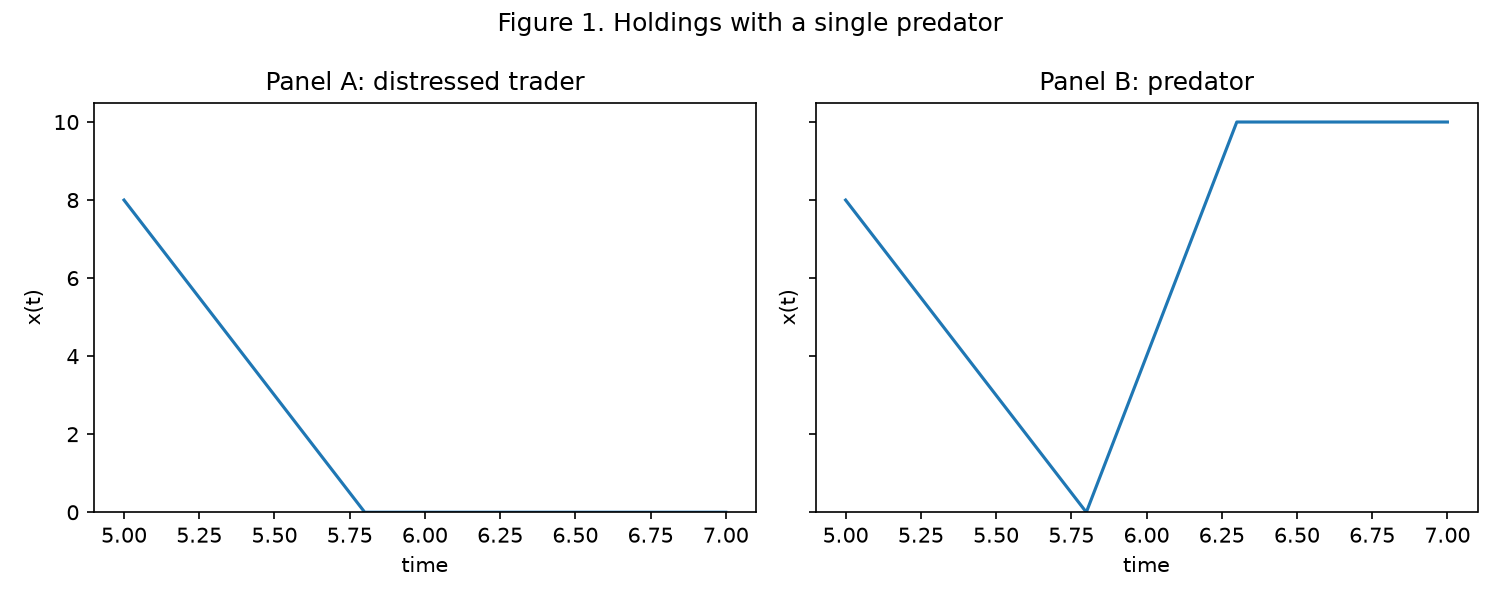
\includegraphics[width=0.62\linewidth]{fig1_holdings.png}\hfill
  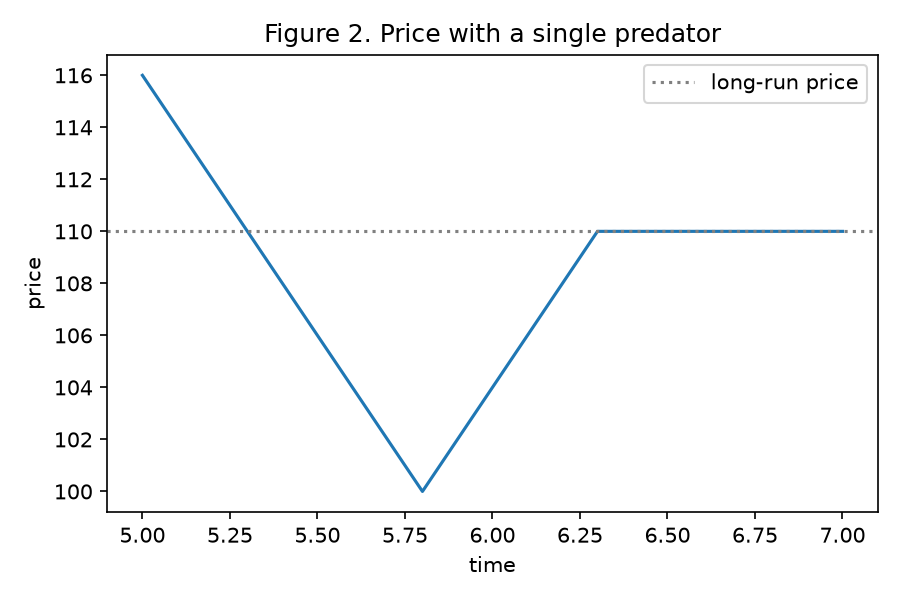
\includegraphics[width=0.36\linewidth]{fig2_price.png}
  \caption{Proposition~1. Left: holdings of the distressed trader and the predator
  (BP Fig.~1). Right: the price falls from 116 to 100 and recovers to 110 (BP Fig.~2).}
  \label{fig:prop1}
\end{figure}

\begin{table}[t]
  \centering\small
  \caption{Proposition~1: our simulation against BP's printed values.}
  \label{tab:prop1}
  \begin{tabular}{@{}lcc@{}}
    \toprule
    Quantity & BP & Simulation \\
    \midrule
    Price at $t = 5$, $5.8$, $6.3$, $7$ & 116, 100, 110, 110 & 116, 100, 110, 110 \\
    Predator's holding at $t = 5.8$ and $6.3$ & 0 and 10 & 0 and 10 \\
    Gain from selling the last share (vs.\ selling one less) & $101.00 - 100.50 = 0.50$ & 0.50 \\
    Paper / orderly / distressed value of the position & ordering only & 928 / 896 / 864 \\
    \bottomrule
  \end{tabular}
\end{table}

The price overshoots its new level of 110 by 10. The striking feature is that the predator
keeps selling even below 110. BP's argument, which our simulation reproduces exactly: the
last share sells at an average of 101.00 and is bought back at an average of 100.50, a
profit of 0.50 over a strategy that sells one share less.

\subsection{Multiple predators (Propositions 2, 2$'$ and 3)}
With several predators a second force appears: each wants to rebuild its position before
the others. In equilibrium (Proposition~2), when
$x(t_0) \ge \frac{I_p - 1}{I - 1}\,\xbar$, predators sell at $A/I$ for
\[
  \tau = \frac{x(t_0) - \frac{I_p - 1}{I - 1}\,\xbar}{A/I},
\]
then buy at $A I_d / (I(I_p - 1))$, a speed that keeps each predator's $X_{-i}$ flat, until
the distressed traders are out. Figure~\ref{fig:prop2} reproduces BP's Figure~3, with a
third of traders distressed, total holdings $I\,x(t_0) = 16$ and total capacity
$I\xbar = 20$. The simulated price equals BP's closed form (eq.~20) at every grid point for
$I = 3$, $9$ and $27$.

\begin{figure}[t]
  \centering
  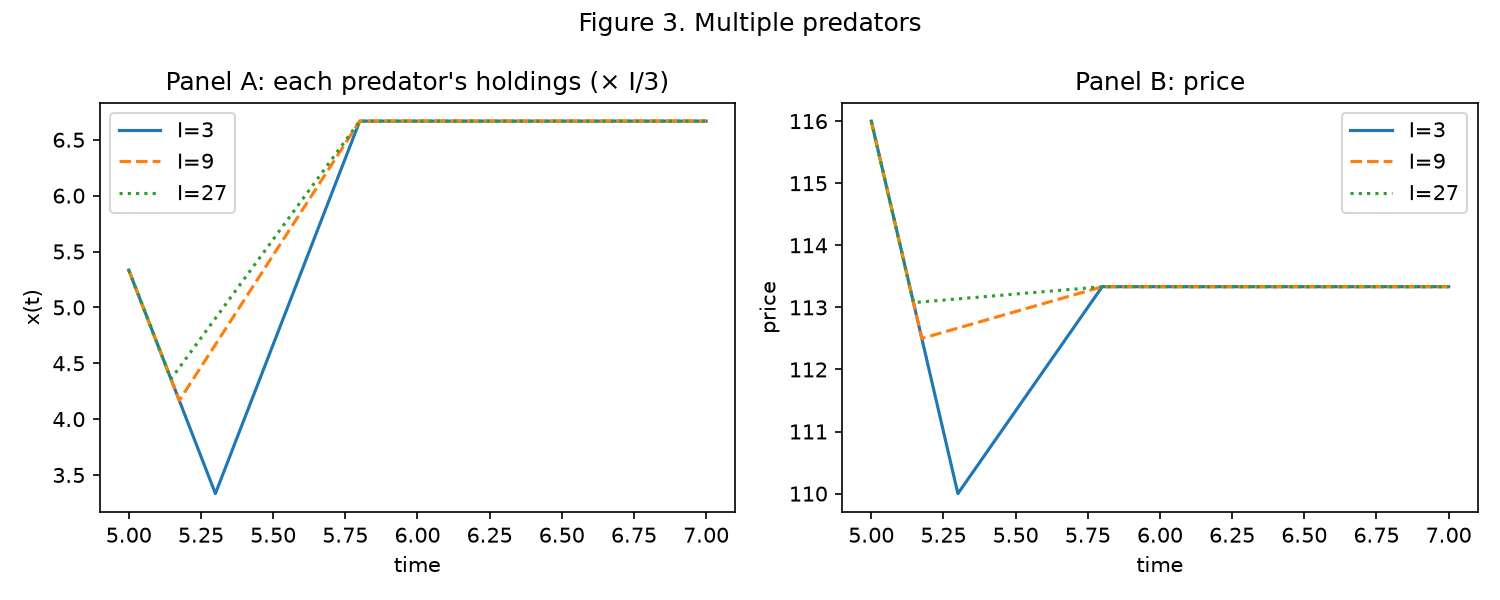
\includegraphics[width=0.66\linewidth]{fig3_multiple_predators.png}\hfill
  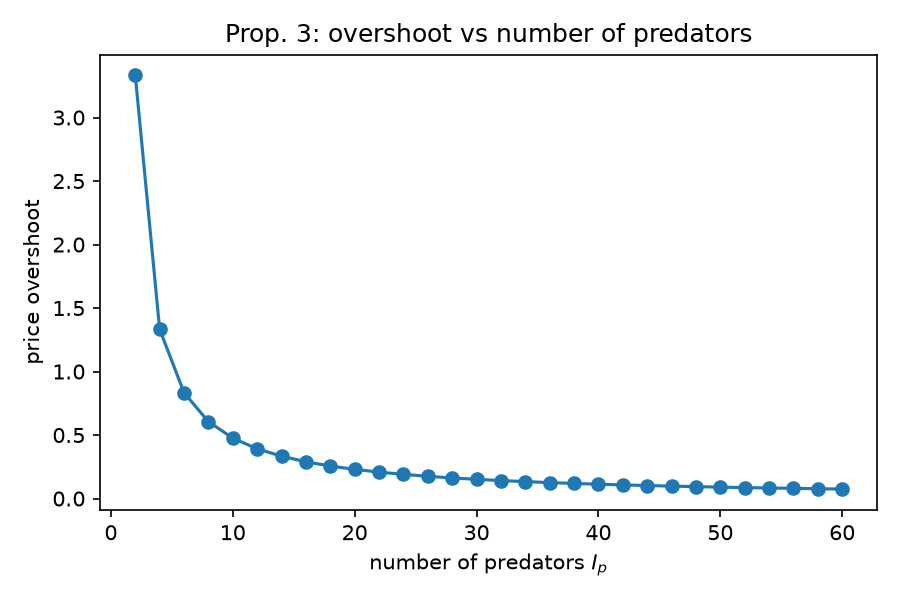
\includegraphics[width=0.33\linewidth]{prop3_overshoot.png}
  \caption{Left: holdings and price with $I = 3, 9, 27$ (BP Fig.~3). Right:
  Proposition~3, the overshoot falls toward zero as predators are added with the total
  holdings fixed.}
  \label{fig:prop2}
\end{figure}

\begin{table}[h]
  \centering\small
  \caption{Overshoot with multiple predators (long-run price 113.33 in every case).}
  \label{tab:prop3}
  \begin{tabular}{@{}rrrr@{}}
    \toprule
    $I$ & Predators $I_p$ & Lowest price & Overshoot \\
    \midrule
    3 & 2 & 110.00 & 3.33 \\
    9 & 6 & 112.50 & 0.83 \\
    27 & 18 & 113.08 & 0.26 \\
    \bottomrule
  \end{tabular}
\end{table}

As Proposition~3 states, the overshoot is positive, falls strictly with the number of
predators, and vanishes in the limit: we find it strictly decreasing for $I = 3,\dots,147$
and below $10^{-3}$ at 20{,}000 predators (Table~\ref{tab:prop3}).

When predators have plenty of spare capacity, $x(t_0) < \frac{I_p - 1}{I - 1}\,\xbar$,
competition to buy dominates and there is no predation (Proposition~2$'$). Predators first
buy at the market's full speed, $A(I + I_d)/(I_p I)$ each, until each $X_{-i}$ reaches its
final level $(I_p - 1)\xbar$, which takes
\[
  \tau' = \frac{(I_p - 1)\xbar - (I - 1)\,x(t_0)}{A\,\bigl(1 - (I + I_d)/(I_p I)\bigr)},
\]
and then absorb exactly the distressed selling. With $I = 3$, $x(t_0) = 4$, $\xbar = 10$, the
price rises steadily from 112 to 120 with no overshoot. These dynamics apply when the
fast-buying phase ends before the distressed traders are out, $t_0 + \tau' \le t_0 +
x(t_0) I/A$ (in this example, $x(t_0) \ge 3.33$); our code checks this condition.

\subsection{Valuation and disclosure (Propositions 5--7)}
BP distinguish three values of a position: the \emph{paper} (mark-to-market) value
$x\,p$, the \emph{orderly} liquidation value $x(p - \lambda x/2)$ from a secret sale, and the
\emph{distressed} liquidation value raised while being preyed upon. Proposition~5 orders them
as paper $>$ orderly $>$ distressed; we confirm this for BP's example ($928 > 896 > 864$) and
the Figure~3 settings. Proposition~6 says more predators raise the distressed value but never
to the orderly value. With $I\,x(t_0) = 18$, the total distressed value rises from 676 with
two predators towards 683.6 with 200, still below the orderly value of 690
(Figure~\ref{fig:val}, left).\footnote{Proposition~6 requires $x(t_0) \ge \xbar\sqrt{I_p/I}$,
which the Figure~3 setting ($I\,x(t_0) = 16$) does not meet, so we use $I\,x(t_0) = 18$.}

Proposition~7 endogenises positions before $t_0$: with probability $\pi$ a random trader
becomes distressed. Traders hold $(1 - \pi/I)\xbar$ if positions are not disclosed and
$(1 - \pi/(I - 1))\xbar$ if they are. Disclosure makes traders hold less (for $I = 5$,
$\pi = 0.5$: 8.75 instead of 9.0), but never little enough to prevent predation
(Figure~\ref{fig:val}, right). This is BP's explanation for hedge-fund secrecy.

\begin{figure}[t]
  \centering
  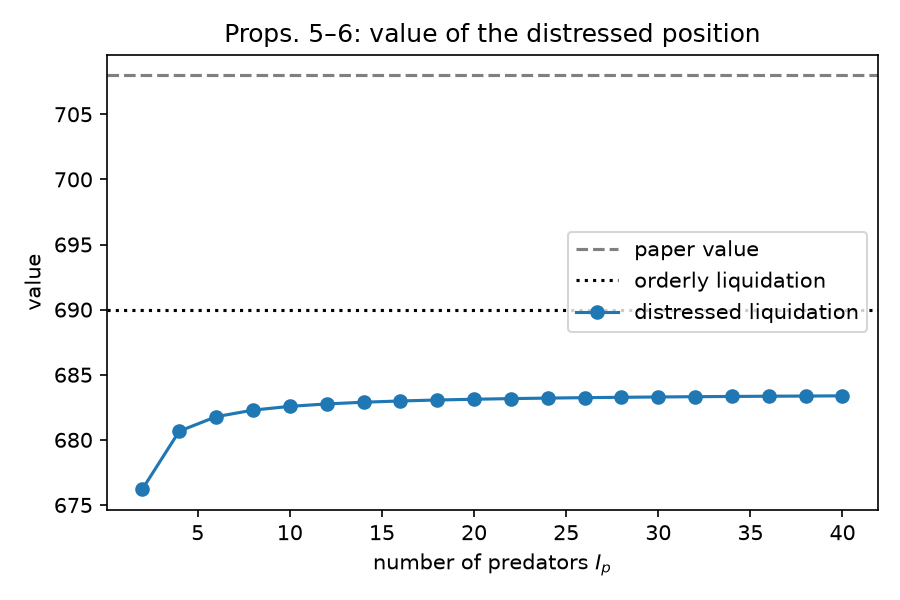
\includegraphics[width=0.45\linewidth]{prop56_valuation.png}\hfill
  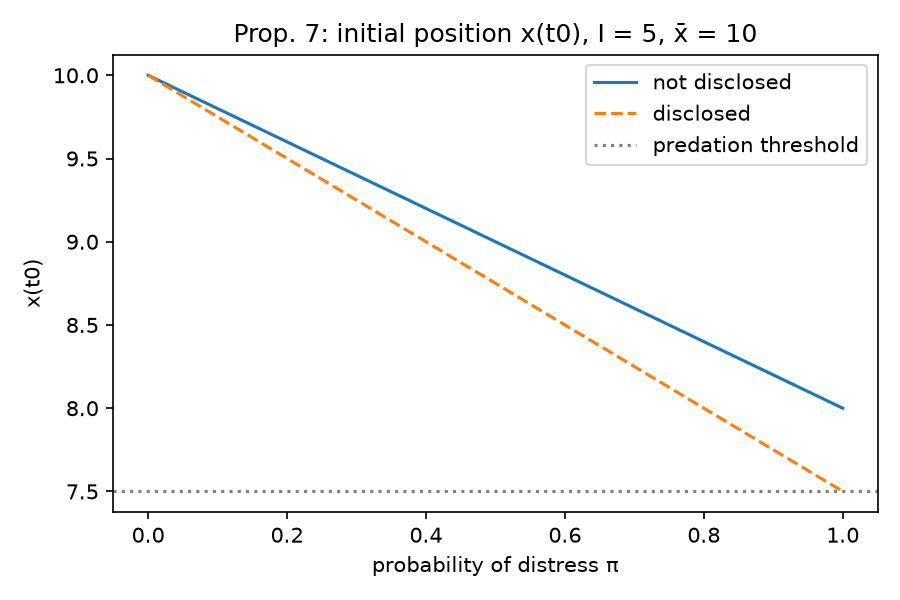
\includegraphics[width=0.45\linewidth]{prop7_disclosure.png}
  \caption{Left: Propositions~5--6, value of the distressed position against the number of
  predators. Right: Proposition~7, initial positions with and without disclosure, against
  the predation threshold.}
  \label{fig:val}
\end{figure}

\subsection{Market design: front-running and batch auctions (Propositions 8--9)}
If the distressed traders only start selling at a later time $t_1$, predators front-run:
they sell first at $A/I_p$ each, wait, and buy back while the distressed traders sell
(Proposition~8). If instead trading is halted and all orders clear in a batch auction at
$t_0$, as with circuit breakers, predators cannot walk down the demand curve and buy part
of their shares in the auction (Proposition~9). Our simulated prices equal BP's closed forms
(eqs.~25--26) at every grid point. Proposition~8's strategy requires each predator's
position during front-running, $x(t_0) - A\tau/I_p$, to stay within $-\xbar$; this holds in
BP's examples and our code checks it.

\begin{figure}[t]
  \centering
  \begin{minipage}{0.55\linewidth}
    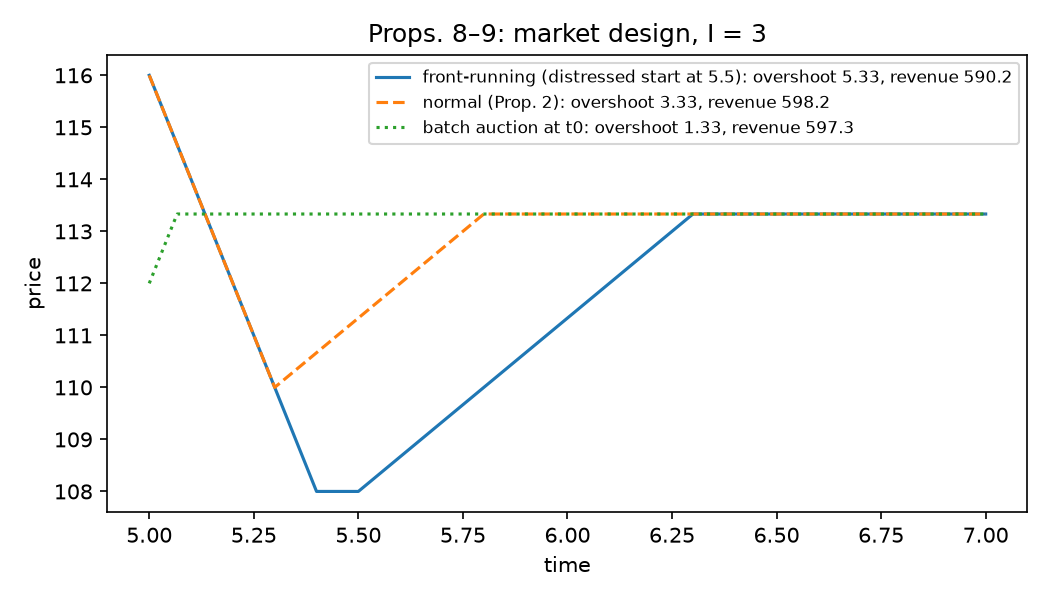
\includegraphics[width=\linewidth]{prop89_market_design.png}
  \end{minipage}\hfill
  \begin{minipage}{0.42\linewidth}
    \small
    \begin{tabular}{@{}lrr@{}}
      \toprule
      Market & Overshoot & Revenue \\
      \midrule
      Front-running & 5.33 & 590.2 \\
      Normal (Prop.~2) & 3.33 & 598.2 \\
      Batch auction & 1.33 & 597.3 \\
      \bottomrule
    \end{tabular}
  \end{minipage}
  \caption{Propositions~8--9 with $I = 3$ (one distressed trader, front-running until
  $t_1 = 5.5$). Revenue is the distressed trader's total proceeds.}
  \label{fig:market}
\end{figure}

Figure~\ref{fig:market} compares the three market designs. Front-running deepens the
overshoot (the price falls to 108) and lowers the distressed trader's revenue, while the
batch auction cuts the overshoot from 3.33 to 1.33. We add one observation: the batch
auction stabilises the price but does \emph{not} raise the distressed seller's revenue. In
continuous trading the seller's first shares fetch prices near 116; in the auction all
shares sell at the single clearing price of 112. With one predator the two effects cancel
exactly (864.0 in both cases); in every multi-predator setting we tried the auction was
slightly worse for the seller (e.g.\ 597.3 against 598.2 here, and 636.0 against 654.0 with
two distressed traders). Circuit breakers calm prices, but their benefit to the trader in
distress is not automatic.

% =========================================================================
\section{Verification}
\label{sec:verification}

\subsection{Best responses as linear programs}
BP derive their equilibria analytically. To check them independently we compute each
predator's best response numerically. Fix every other trader's strategy; then $X_{-i}$ is
fixed, and by Lemma~1 trader $i$'s payoff on our grid is a constant minus
\[
  \lambda \sum_k a_k\,dt\,\frac{X_{-i,k} + X_{-i,k+1}}{2},
\]
which is linear in the trader's trades. The best response is therefore a linear program,
and its optimum is exact for the discretised game. We take the trader's holdings
$x_0,\dots,x_N$ as variables, so the position limit becomes simple bounds, the speed caps
become a sparse two-band constraint on $x_{k+1} - x_k$, and $x_0 = x(t_0)$, $x_N = \xbar$
are fixed. With 2{,}000 steps each LP solves in 10--30 ms with HiGHS \cite{highs}.

\begin{table}[t]
  \centering\small
  \caption{Payoff of the last predator: BP's strategy against the best possible response,
  everyone else held at BP's strategy.}
  \label{tab:lp}
  \begin{tabular}{@{}lrr@{}}
    \toprule
    Case & BP's strategy & Best response (LP) \\
    \midrule
    Proposition 1 & 1214.000000 & 1214.000000 \\
    Proposition 2, $I = 3$ & 787.111111 & 787.111111 \\
    Proposition 2, $I = 9$ & 261.444444 & 261.444444 \\
    Proposition 2$'$, $I = 3$, $x(t_0) = 4$ & 702.000000 & 702.000000 \\
    Proposition 8, $I = 3$, $t_1 = 5.5$ & 791.111111 & 791.111111 \\
    \bottomrule
  \end{tabular}
\end{table}

Table~\ref{tab:lp} shows that no predator can improve on BP's strategy: the best response
pays exactly the same, to six decimal places, in every case (our tests check every predator,
not only the last). The best response need not coincide with BP's strategy, since BP note
that the buy-back speed is free (their footnote~13); but the tests confirm the part that is
pinned down, such as the predator's position when the selling stops. Two further checks
show the comparison is meaningful. A predator that simply buys from $t_0$ gains more than 1
by switching to the LP's strategy. And if the speed caps are removed, the LP earns 1324
instead of 1214, so the check would detect a wrong speed limit. Finally, solving the LP for
every end position from $-\xbar$ to $\xbar$ confirms Lemma~1's premise that ending at
$\xbar$ is optimal: the best payoff rises all the way to $\xbar$ (from 414 to 1214 in
Proposition~1).

\subsection{Learning the equilibrium}
Is the predatory equilibrium only a fixed point, or would traders find it? We start the
predators on a naive strategy, simply buying steadily while the distressed traders sell,
and let them respond to each other.

Plain best-response iteration cycles: the overshoot jumps between 12 and 26 for twelve rounds
without settling ($I = 3$ and $9$), because best responses are all-or-nothing (against an exploitable opponent
a predator dumps its position at full speed). We therefore use fictitious play
\cite{brown1951,robinson1951}: in round $k$ each predator moves a step $1/(k + 2)$ toward its
best response, i.e.\ it plays the average of its past best responses. Because BP's
Proposition~2 is the unique \emph{symmetric} equilibrium, we let all predators share one
strategy (one LP per round).

\begin{figure}[t]
  \centering
  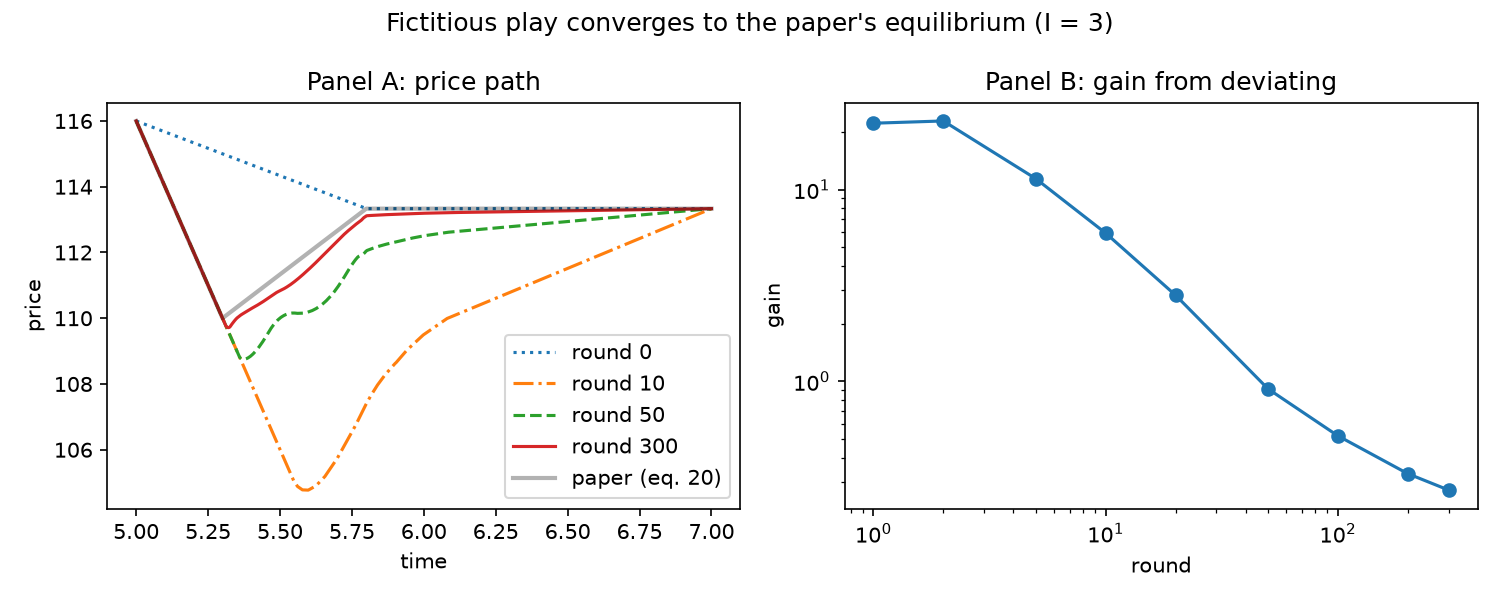
\includegraphics[width=0.85\linewidth]{fictitious_play.png}
  \caption{Fictitious play from a naive start ($I = 3$). Left: price paths. Predators first
  learn to prey and overdo it (round 10), then converge to BP's path. Right: the most any
  predator could gain by deviating, on log scales.}
  \label{fig:fp}
\end{figure}

\begin{table}[h]
  \centering\small
  \caption{Fictitious play: largest distance from BP's price path (eq.~20) and gain from
  deviating.}
  \label{tab:fp}
  \begin{tabular}{@{}rrrrr@{}}
    \toprule
    & \multicolumn{2}{c}{$I = 3$} & \multicolumn{2}{c}{$I = 9$} \\
    \cmidrule(lr){2-3}\cmidrule(lr){4-5}
    Round & Price gap & Gain & Price gap & Gain \\
    \midrule
    1 & 13.33 & 22.22 & 13.33 & 65.81 \\
    10 & 7.27 & 5.93 & 14.51 & 19.95 \\
    50 & 1.89 & 0.91 & 4.36 & 3.25 \\
    200 & 0.61 & 0.33 & 1.66 & 0.94 \\
    1000 & 0.24 & 0.13 & 0.53 & 0.30 \\
    \bottomrule
  \end{tabular}
\end{table}

Figure~\ref{fig:fp} and Table~\ref{tab:fp} show the result. At round 0 there is no
predation. By round 10 the predators have learned to prey but overdo it, and the price falls
to about 105, far below BP's 110. From there the path tightens onto BP's, and the gain from
deviating falls steadily (roughly like $1/k$, typical of fictitious play). When each
predator instead keeps its own strategy and starts from a different one, both still converge
to the symmetric equilibrium (positions at $t_0 + \tau$ of 3.335 and 3.323 after 300 rounds,
against 3.333 each), consistent with BP's uniqueness result. \emph{Predation is not only an
equilibrium: traders who merely respond to each other discover it.}

Averaging strategies can make the market as a whole trade faster than $A$: with six
predators in round 1, each adopts a response that was feasible only if the others stayed
put. This is why the simulator charges the impact cost $\gamma$ for excess trading
(Section~\ref{sec:discrete}); the figures above include it. Since a trader can exceed its
cap only if the whole market trades faster than $A$, the caps need computing only at such
steps, so equilibrium simulations pay nothing for this.

% =========================================================================
\section{Extensions}
\label{sec:extensions}

\subsection{Collusion}
BP note that colluding predators would ``jointly act like a single predator'', selling
until the distressed traders are out and only then rebuilding, and that tacit collusion
cannot arise in their model. We build the cartel in two independent ways and check that
they agree. In closed form, each predator sells at $A/I$ alongside the distressed traders,
then all rebuild at $A/I_p$ each. Numerically, Lemma~1's algebra applies to the group's
total holdings, so the cartel solves one linear program for a single trader with capacity
$I_p\xbar$ facing only the distressed traders. The two match to $10^{-6}$.

\begin{figure}[t]
  \centering
  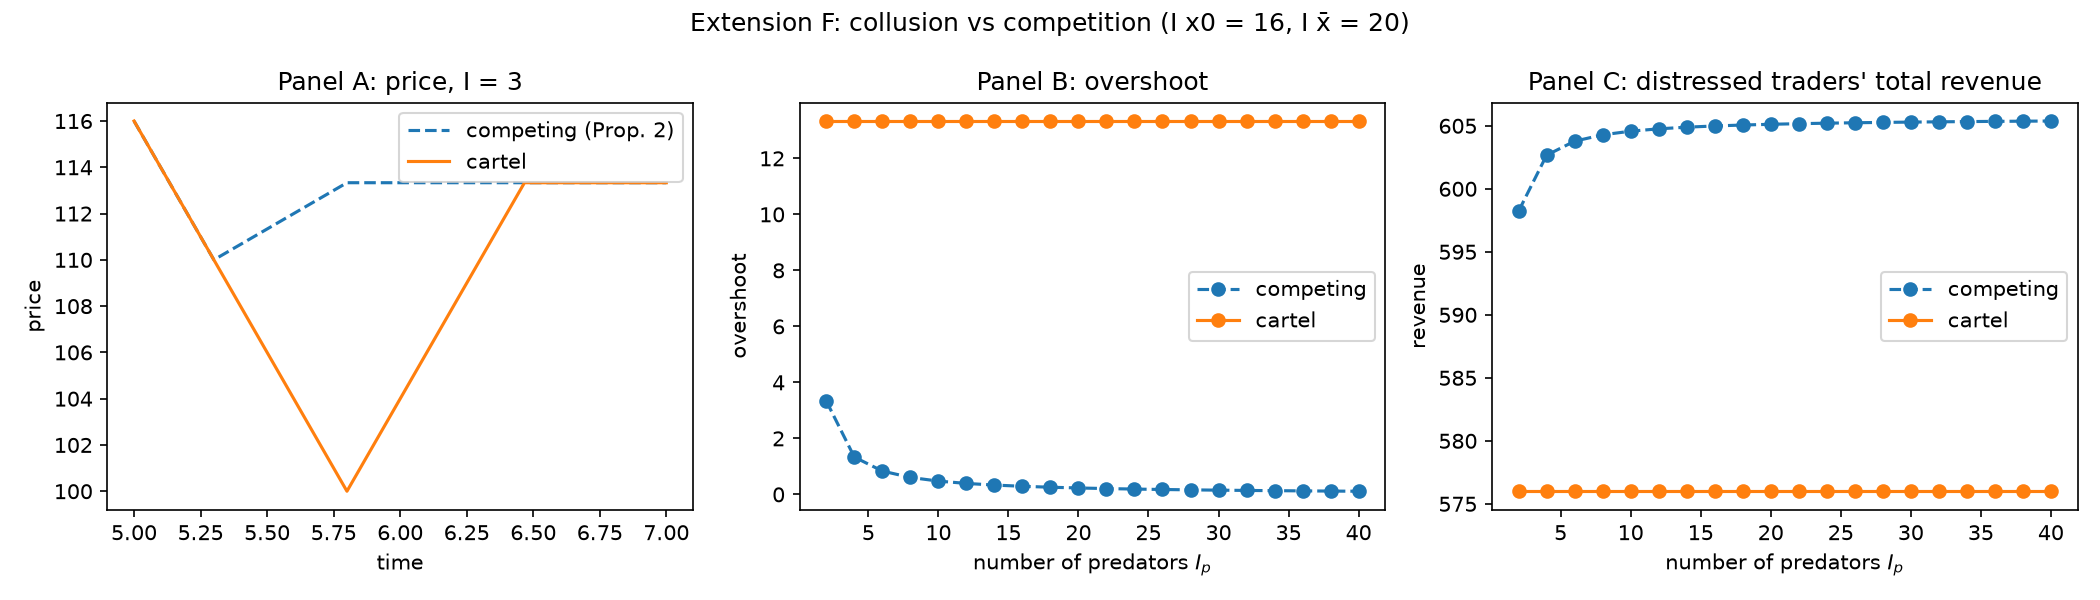
\includegraphics[width=\linewidth]{collusion.png}
  \caption{Collusion against competition with BP's Figure~3 totals. A cartel keeps an
  overshoot of 13.33 whatever its size, while competition erodes it.}
  \label{fig:collusion}
\end{figure}

\begin{table}[h]
  \centering\small
  \caption{Competing predators against a cartel.}
  \label{tab:collusion}
  \begin{tabular}{@{}rrrrr@{}}
    \toprule
    $I$ & Overshoot & Distressed revenue & Predators' total payoff & Gain from cheating \\
    \midrule
    3 & 3.33 $\to$ 13.33 & 598.22 $\to$ 576.00 & 1574.22 $\to$ 1596.44 & 16.67 (2.1\%) \\
    9 & 0.83 $\to$ 13.33 & 603.78 $\to$ 576.00 & 1568.67 $\to$ 1596.44 & 11.34 (4.3\%) \\
    27 & 0.26 $\to$ 13.33 & 605.06 $\to$ 576.00 & 1567.38 $\to$ 1596.44 & --- \\
    \bottomrule
  \end{tabular}
\end{table}

Figure~\ref{fig:collusion} and Table~\ref{tab:collusion} give four results.
\begin{itemize}
  \item \textbf{The cartel's overshoot does not shrink with its size.} It always sells down
        to $\mu - \lambda S = 100$, so the overshoot is $\lambda I_p \xbar = 13.33$ however
        many members it has, whereas competition drives the overshoot toward zero.
  \item \textbf{Collusion is a pure transfer.} The predators gain exactly what the
        distressed traders lose (22.22 with $I = 3$, 27.78 with $I = 9$); long-term investors
        are unaffected, as BP remark.
  \item \textbf{Collusion is unstable.} A member gains by rebuilding early, before the
        others, confirming numerically that collusion is not an equilibrium. The temptation
        is a larger share of a member's profit in a larger cartel (2.1\% with two members,
        4.3\% with six), the usual reason large cartels are hard to sustain.
  \item \textbf{A cartel preys even where competition would provide liquidity.} With
        spare capacity ($I = 3$, $x(t_0) = 4$, $\xbar = 10$), competing predators buy at once
        and there is no overshoot (Proposition~2$'$), but a cartel still sells first and the
        price goes $112 \to 100 \to 120$, an overshoot of 12.
\end{itemize}
Repeated interaction, in which a cartel could punish cheaters and sustain tacit collusion,
is outside the model; Carlin, Lobo and Viswanathan \cite{clv2007} study it.

\subsection{Contagion}
BP's Section~III.B endogenises distress. A trader must liquidate if its wealth falls to a
threshold $\underline W$. Its survival hurdle $W(I_d)$ is the highest wealth at $t_0$ at
which it \emph{cannot} avoid distress if $I_d$ traders, itself included, are expected to
fail (BP eq.~21), and Proposition~4 states that $W(I_d)$ increases with $I_d$. BP illustrate
the resulting contagion with a stylised figure but do not compute the hurdles.

\paragraph{Definition.} We make eq.~(21) concrete. The other traders are $I_d - 1$ distressed
traders and $I_p$ predators playing the $I_d$-distressed equilibrium. Wealth is
mark-to-market, $W_i = x_i\,p + \text{cash} + \text{other assets}$, and on our grid its change
over a step is exactly $\lambda[\tfrac12(x_{k+1}^2 - x_k^2) + \bar x_k\,\Delta X_{-i,k}]$,
with $\bar x_k$ the average holding over the step. Then
\[
  W(I_d) = \underline W + D(I_d), \qquad
  D(I_d) = -\max_{a_i}\,\min_t\,\Delta W_i(t),
\]
the smallest worst-case drop trader $i$ can achieve with \emph{any} strategy.

\paragraph{Computation.} The $x^2$ term makes this max--min problem non-convex. We solve it by
sequential linear programming, a convex--concave procedure \cite{lipp2016}: replace
$\tfrac12 x^2$ by its tangent at the current path (never above it, so every LP solution is
truly achievable), solve the LP, re-linearise at the new path and repeat. Each step can only
improve, and we run it from several starting paths. In experiments, 25 random starting paths
per $I_d$ all reached the same values, and the values are identical at $dt = 0.005$,
$0.0025$ and $0.001$.

\paragraph{Results.} We use six traders A--F as in BP's Figure~4 ($\xbar = 6$,
$x(t_0) = 5$, $T = 9$, other parameters as before).

\begin{table}[h]
  \centering\small
  \caption{Survival hurdles above the threshold, $D(I_d) = W(I_d) - \underline W$.}
  \label{tab:hurdles}
  \begin{tabular}{@{}lrrrrrr@{}}
    \toprule
    $I_d$ & 1 & 2 & 3 & 4 & 5 & 6 \\
    \midrule
    Any strategy (eq.~21) & 0 & 27 & 48 & 63 & 72 & 72 \\
    Selling or holding only & 5 & 34.5 & 57 & 70.5 & 75 & 75 \\
    \bottomrule
  \end{tabular}
\end{table}

Table~\ref{tab:hurdles} confirms Proposition~4 under both rules: the more failures expected,
the fiercer the predation and the higher the hurdle (strictly up to $I_d = 5$; from 5 to 6 it
is flat, because a lone predator sells alongside the distressed traders just as a sixth
distressed trader would). The optimal survival strategy is notable: \textbf{sell at the speed
limit for a while, then buy hard as the price bottoms}. The trader's own buying props up the
price, and with it the paper value of its holdings, exactly when its wealth would otherwise
be lowest. This mirrors the distressed trader who buys to support the price in Attari, Mello
and Ruckes \cite{amr2005}. It matters: with $I_d = 4$ the best strategy limits the drop to 63,
against 95 for holding and 71 for selling out. We therefore report both the literal eq.~(21)
hurdles and a variant in which a trader in trouble may only sell or hold.

\begin{figure}[t]
  \centering
  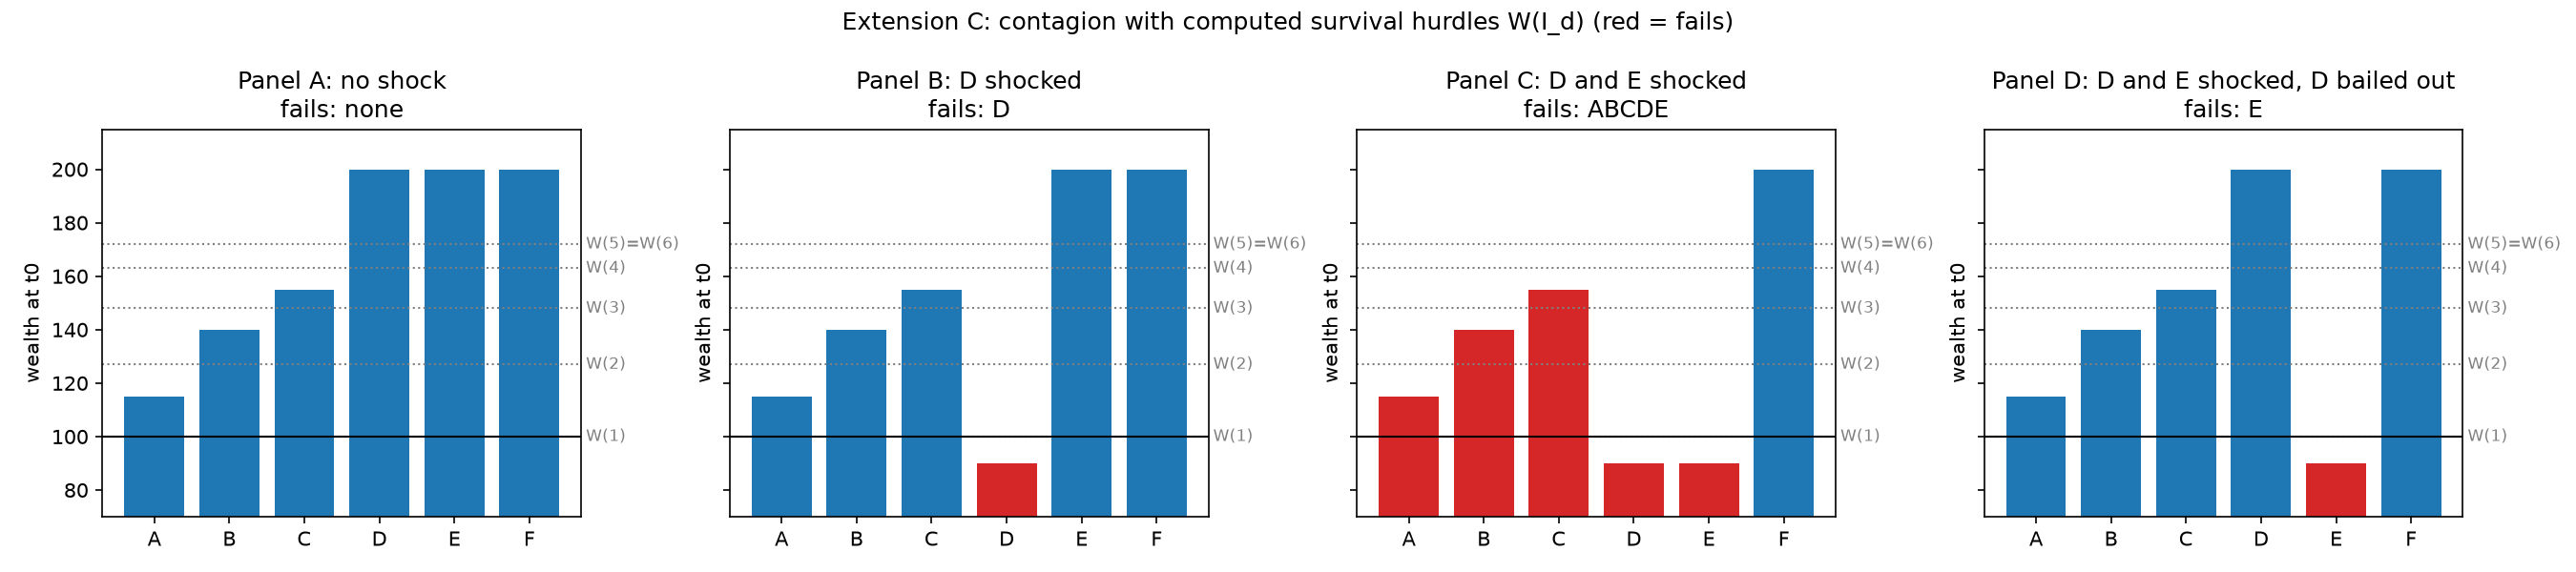
\includegraphics[width=\linewidth]{contagion.png}
  \caption{Contagion with the computed hurdles ($\underline W = 100$, so
  $W(1),\dots,W(6) = 100, 127, 148, 163, 172, 172$). Red bars fail.}
  \label{fig:contagion}
\end{figure}

An outcome with $I_d$ failures is consistent if exactly the $I_d$ traders with wealth at most
$W(I_d)$ fail. The \emph{ripple} starts from the traders forced out and adds those who fall
below the hurdle for the current number of failures. With wealth levels placed as in BP's
Figure~4 (A, B and C between consecutive hurdles; D, E and F safe), Figure~\ref{fig:contagion}
shows four scenarios.
\begin{itemize}
  \item \textbf{No shock:} the only consistent outcome is no failure.
  \item \textbf{D shocked:} 1, 2, 3 or 4 failures are all consistent. If the market expects
        four failures, predation is fierce enough to cause them: a panic. Without panic only
        D fails.
  \item \textbf{D and E shocked:} the unique outcome is the ripple D, E $\to$ A $\to$ B $\to$ C,
        exactly as BP describe.
  \item \textbf{D and E shocked, D bailed out:} only E fails. Recapitalising one trader
        stops the cascade, BP's argument for central-bank intervention.
\end{itemize}

\subsection{Predators with unequal positions}
BP's footnote~15 describes, in words, the equilibrium when predators start with different
positions: everyone sells at $A/I$ until the $X_{-i}$ of the predator with the
\emph{smallest} position reaches its final level $(I_p - 1)\xbar$, at a time $s$; then
predators buy at $I_d A / (I(m - 1))$ each, where $m$ is the number still buying, and speed
up as others finish. For the last remaining buyer we take the natural reading that it waits
until the distressed traders are out and then buys at the full speed $A$. We build this
strategy step by step, and the LP solver confirms it is an equilibrium (no profitable
deviation, to $10^{-6}$) for two predators at $x(t_0) \pm 0.5$ and $\pm 1$, and for three
predators at $x(t_0) - \delta, x(t_0), x(t_0) + \delta$ with $\delta = 0.4$ and $0.8$, which
exercises the speed-up rule. With equal positions it reduces exactly to Proposition~2.

\begin{figure}[t]
  \centering
  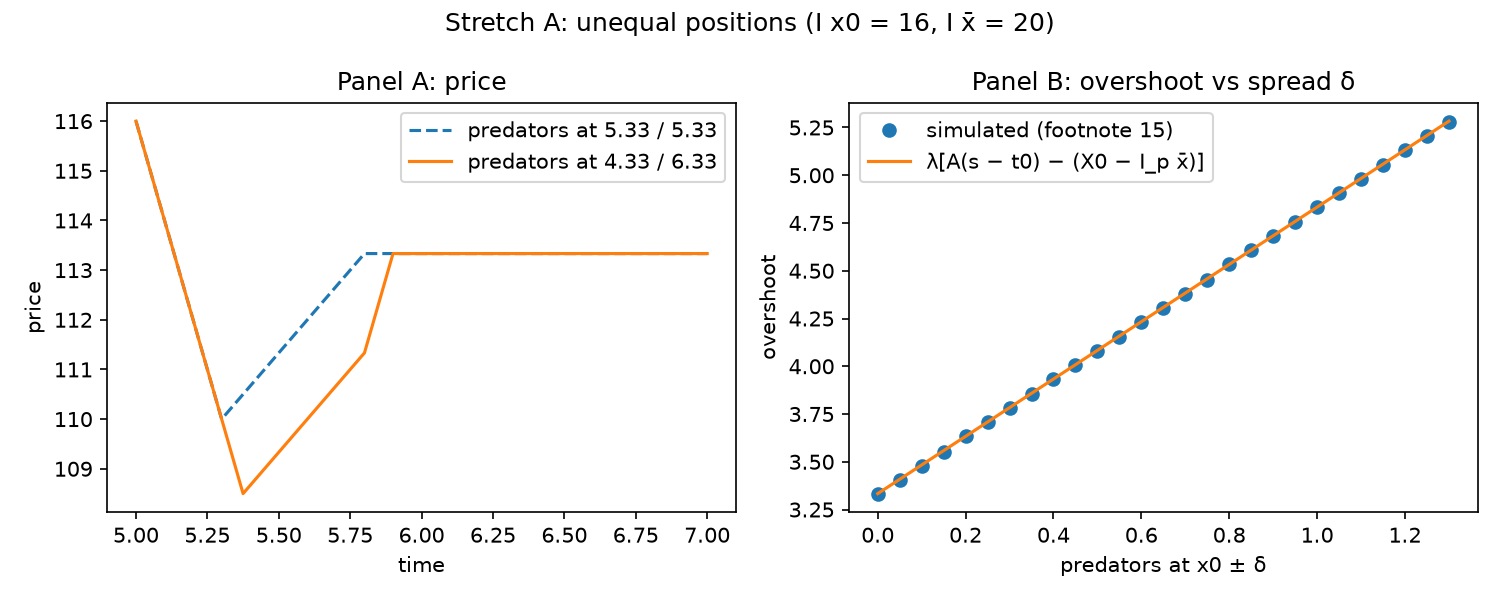
\includegraphics[width=0.85\linewidth]{unequal_positions.png}
  \caption{Unequal predator positions, $I = 3$. Left: a smaller predator prolongs the selling
  and deepens the trough. Right: the simulated overshoot lies exactly on
  equation~\eqref{eq:unequal}.}
  \label{fig:unequal}
\end{figure}

BP state that, for fixed total holdings, overshooting increases with the dispersion of
predators' initial positions. The mechanism yields a sharper statement. The price troughs
at $s$, and $s$ depends on the positions only through the smallest predator's,
$x_{\min}$, and the total $X_0$:
\begin{equation}
  \text{overshoot} = \lambda\bigl[A(s - t_0) - (X_0 - I_p\xbar)\bigr], \qquad
  s - t_0 = \frac{\bigl(X_0 - x_{\min} - (I_p - 1)\xbar\bigr)\,I}{(I - 1)\,A}.
  \label{eq:unequal}
\end{equation}
The overshoot rises by $\lambda I/(I - 1)$ for each unit the smallest position sits below
the rest, and the rest of the dispersion is irrelevant: \textbf{only the smallest predator
matters}. It has the most of everyone else's selling still ahead of it, so it keeps selling
longest, and everyone keeps selling with it. With $I = 3$ the overshoot is $3.33$, $4.08$,
$4.83$ for spreads $\delta = 0, 0.5, 1$; with $I = 4$, predators at $(3.2, 4.0, 4.8)$ and at
$(3.2, 4.4, 4.4)$ have different dispersion but the same smallest position and give exactly
the same overshoot, $41/15 \approx 2.733$ (Figure~\ref{fig:unequal}).

% =========================================================================
\section{Limitations and future work}
\begin{itemize}
  \item \textbf{Distressed traders follow BP's rule.} Best responses are computed for
        predators only; a distressed trader's obligation to sell while holding shares
        depends on its own position and is not a fixed linear constraint.
  \item \textbf{Fictitious play converges slowly}, roughly like $1/k$, so its results are
        reported with tolerances.
  \item \textbf{Contagion is one-shot.} The cascade uses wealth at $t_0$, following BP's
        logic; wealth is not re-simulated as traders fail. The hurdle computation finds a
        local optimum; multiple starts make a missed better strategy unlikely but this is
        not a proof.
  \item \textbf{Time-varying liquidity.} If $\lambda$ rises during a crisis, a trader's own
        price impact no longer cancels and Lemma~1's linear structure is lost; the
        sequential-LP approach of the contagion section is a natural route.
  \item \textbf{Empirical calibration.} Estimating $\lambda$ and $A$ from intraday data, or
        testing the overshoot-and-recovery pattern around index rebalances or crypto
        liquidations, would connect the model to data.
\end{itemize}

% =========================================================================
\section{Conclusion}
We implemented Brunnermeier and Pedersen's model of predatory trading as an exact
discrete-time simulation and reproduced its propositions and figures. Linear-programming best
responses confirm that no predator can improve on the paper's strategies, and fictitious play
shows that traders starting without predation learn it. Extending the analysis, we found that
a cartel sustains a large overshoot regardless of its size but is unstable; that the best way
for a trader in trouble to survive is to sell and then buy at the bottom, and that with
computed survival hurdles one trader's distress can ripple through the market unless a
bailout stops it; and that with unequal positions the overshoot is governed by the smallest
predator alone. The results support BP's policy lessons: liquidity vanishes when it is most
needed, secrecy protects large traders, circuit breakers calm prices, and bailouts can halt
cascades.

% =========================================================================
\begin{thebibliography}{9}
\bibitem{bp2005} M.~K. Brunnermeier and L.~H. Pedersen. Predatory trading.
  \emph{Journal of Finance}, 60(4):1825--1863, 2005.
\bibitem{clv2007} B.~I. Carlin, M.~S. Lobo and S.~Viswanathan. Episodic liquidity crises:
  cooperative and predatory trading. \emph{Journal of Finance}, 62(5):2235--2274, 2007.
\bibitem{amr2005} M.~Attari, A.~S. Mello and M.~E. Ruckes. Arbitraging arbitrageurs.
  \emph{Journal of Finance}, 60(5):2471--2511, 2005.
\bibitem{brown1951} G.~W. Brown. Iterative solution of games by fictitious play. In
  \emph{Activity Analysis of Production and Allocation}, Wiley, 1951.
\bibitem{robinson1951} J.~Robinson. An iterative method of solving a game.
  \emph{Annals of Mathematics}, 54(2):296--301, 1951.
\bibitem{lipp2016} T.~Lipp and S.~Boyd. Variations and extension of the convex--concave
  procedure. \emph{Optimization and Engineering}, 17:263--287, 2016.
\bibitem{highs} Q.~Huangfu and J.~A.~J. Hall. Parallelizing the dual revised simplex method.
  \emph{Mathematical Programming Computation}, 10(1):119--142, 2018.
\end{thebibliography}

% =========================================================================
\appendix
\section{Code and reproducibility}
The project is at \url{https://github.com/dudegladiator/predatory-trading}. It uses Python
3.13 managed with \texttt{uv}; NumPy, SciPy (HiGHS linear programming), Matplotlib and
Streamlit.

\begin{center}\small
\begin{tabular}{@{}ll@{}}
  \toprule
  File & Contents \\
  \midrule
  \texttt{src/model.py} & Parameters, price, speed caps, impact cost, simulator \\
  \texttt{src/closed\_form.py} & BP's equilibria (Props.~1--9), valuations, the cartel \\
  \texttt{src/solver.py} & LP best responses, cartel LP, fictitious play \\
  \texttt{src/contagion.py} & Survival hurdles by sequential LP, equilibria, cascades \\
  \texttt{src/unequal.py} & Footnote~15 with unequal positions \\
  \texttt{app.py} & Interactive app, one page per result \\
  \texttt{figures.py} & All figures in this report \\
  \texttt{tests/} & 115 automated tests \\
  \bottomrule
\end{tabular}
\end{center}

\noindent Commands: \texttt{uv run pytest} runs the tests (about 30\,s);
\texttt{uv run python figures.py} regenerates the figures; \texttt{uv run streamlit run
app.py} starts the app. Every numerical claim in this report is checked by a test against
BP's printed values or against an independent method (closed form against LP, simulator
against wealth formula, and so on).

\end{document}
